\documentclass[14pt,hidelinks]{extarticle}

\usepackage[T2A]{fontenc}
\usepackage[utf8]{inputenc}
\usepackage[russian]{babel}
\usepackage{cmap}

\usepackage{xcolor}

\usepackage{helvet}
\usepackage{pscyr}


\usepackage{multicol}

% \usepackage{amssymb,amsfonts,amsmath,mathtext}
% \usepackage{cite,enumerate,float}

\graphicspath{{images/}}     % Подключаемые пакеты
%%% Макет страницы %%%
\geometry{a4paper,top=20mm,bottom=27mm,left=30mm,right=15mm}
\setstretch{1.15}

%%% Язык текста %%%
\selectlanguage{russian}

%%% Кодировки и шрифты %%%
\renewcommand{\rmdefault}{ftm} % Включаем Times New Roman

%%% Выравнивание и переносы %%%
\sloppy				% Избавляемся от переполнений
\clubpenalty=10000		% Запрещаем разрыв страницы после первой строки абзаца
\widowpenalty=10000		% Запрещаем разрыв страницы после последней строки абзаца
\interfootnotelinepenalty=10000 % Запрет разрывов сносок

%%% Нумерация страниц %%%
\fancypagestyle{empty}{%
\fancyhf{} % clear all header and footer fields
\renewcommand{\headrulewidth}{0pt}
\renewcommand{\footrulewidth}{0pt}
\setlength{\headheight}{5mm} 
}

\fancypagestyle{plain}{%
\fancyhf{} % clear all header and footer fields
\fancyfoot[R]{\thepage} 
\renewcommand{\headrulewidth}{0pt}
\renewcommand{\footrulewidth}{0pt}
\setlength{\headheight}{5mm}
}

\pagestyle{plain}

%%% Библиография %%%

\makeatletter
\bibliographystyle{ugost2003s} % Оформляем библиографию в соответствии с ГОСТ 7.1 2003

\let\oldthebibliography=\thebibliography
\let\endoldthebibliography=\endthebibliography
\renewenvironment{thebibliography}[1]{
  \begin{oldthebibliography}{#1}
    \setlength{\parskip}{0mm}
    \setlength{\itemsep}{0mm}
}
{
\end{oldthebibliography}
}

%%% Изображения %%%
\graphicspath{{images/}} % Пути к изображениям

%%% Содержание %%%
\renewcommand{\cfttoctitlefont}{\hfil \large\bfseries}

\setlength{\cftparskip}{0mm}
\setlength{\cftbeforesecskip}{0mm}
\setlength{\cftaftertoctitleskip}{14pt}

\renewcommand{\cftsecaftersnumb}{\:}
\renewcommand{\cftsecfont}{}   
\renewcommand{\cftsecpagefont}{\normalsize}
\renewcommand{\cftsecleader}{\cftdotfill{\cftdotsep}}
\setlength{\cftsecindent}{0mm}
\setlength{\cftsecnumwidth}{3mm}

\setlength{\cftsubsecindent}{4mm}
\setlength{\cftsubsecnumwidth}{8mm}

%%% Требования ЕСКД/СТП %%%

%%% Размеры заголовков
\newcommand{\sectionbreak}{\clearpage}

\titleformat{\section}{\large\bfseries}{\thesection}{\wordsep}{}
\titlespacing*{\section}{12mm}{14pt}{14pt}

\titleformat{name=\section,numberless}{\large\bfseries\filcenter}{}{0mm}{}
\titlespacing*{name=\section,numberless}{0mm}{14pt}{14pt}

\titleformat{name=\subsection}{\normalsize\bfseries}{\thesubsection}{\wordsep}{}
\titlespacing*{\subsection}{12mm}{14pt}{14pt}

\titleformat{name=\subsection,numberless}{\normalsize\bfseries}{}{0mm}{}
\titlespacing*{name=\subsection,numberless}{0mm}{14pt}{14pt}

%%% Нумерация параграфов

\counterwithout{paragraph}{subsubsection}
\counterwithin{paragraph}{subsection}
\renewcommand{\theparagraph}{\thesubsection.\arabic{paragraph}}
\setcounter{secnumdepth}{4}

\titleformat{name=\paragraph}[runin]{\normalsize\bfseries}{\theparagraph}{\wordsep}{}
\titlespacing*{\paragraph}{12mm}{14pt}{\wordsep}

%%% Размеры текста формул %%%

\DeclareMathSizes{12}{12}{6}{4}

%%% Расстояние между формулами

\AtBeginDocument{%
  \setlength\abovedisplayskip{14pt}%
  \setlength\belowdisplayskip{14pt}%
  \setlength\abovedisplayshortskip{14pt}%
  \setlength\belowdisplayshortskip{14pt}%
}

%%% Оформление текста

\setlength{\parskip}{0pt}
\setlength{\parindent}{12mm}

%%% Расстояние между плавающими элементами

\setlength{\floatsep}{14pt}     % between top floats
\setlength{\textfloatsep}{14pt} % between top/bottom floats and text
\setlength{\intextsep}{14pt}    % between text and float
\setlength{\dbltextfloatsep}{14pt}
\setlength{\dblfloatsep}{14pt}

 % костыль для того, чтобы убрать расстояние от картинки до текста
\setlength{\abovecaptionskip}{0pt}
\setlength{\belowcaptionskip}{0pt}
           
%%% Оформление списков
\AddEnumerateCounter{\asbuk}{\@asbuk}{\cyrm}

\setlist{nosep,listparindent=\parindent}
\setlist[1]{itemindent=18.5mm,leftmargin=0mm,itemsep=0mm,topsep=0mm,parsep=0mm}             
\setlist[itemize,1]{label=$-$}
\setlist[enumerate,1]{label=\arabic*)}

\setlist[2]{itemindent=20.5mm,leftmargin=0mm,itemsep=0mm,topsep=0mm,parsep=0mm}             

% Определяем новый стиль для списков,
% на которые есть ссылки в тексте
\newlist{reflist}{enumerate*}{1}
\setlist*[reflist,1]{%
  label=\asbuk*),
}

\setlist*[reflist,2]{%
  label=\arabic*),
}

%% Нумерация плавающих элементов

\counterwithin{figure}{section}
\counterwithin{table}{section}

\makeatletter
\AtBeginDocument{%
\renewcommand{\thetable}{\thesection.\arabic{table}}
\renewcommand{\thelstlisting}{\thesection.\arabic{lstlisting}}
\renewcommand{\thefigure}{\thesection.\arabic{figure}}
\let\c@lstlisting\c@figure}
\makeatother 

%% Подписи плавающих элементов

\captionsetup[figure]{
  labelsep=endash,
  justification=centering,
  singlelinecheck=false,
  position=bottom,
  skip=14pt}

\captionsetup[table]{
  labelsep=endash,
  justification=raggedright,
  singlelinecheck=false,
  position=top,
  skip=0mm}

\captionsetup[lstlisting]{
  labelsep=endash
}

\lstset{
basicstyle=\scriptsize\ttfamily,
numberstyle=\scriptsize\ttfamily,
keywordstyle=\bfseries,
commentstyle=\itshape,
numbers=left,
stepnumber=1,
frame=single,
resetmargins=true,
xleftmargin=7mm,
xrightmargin=2mm,
captionpos=b,
keepspaces=true,
breaklines=true,
aboveskip=22pt,
belowskip=10pt,
abovecaptionskip=16pt}

\renewcommand{\arraystretch}{1.5}

%%% Настройка размеров вертикальных отступов

\renewcommand{\smallskip}{\vspace{6pt}}
\renewcommand{\bigskip}{\vspace{14pt}}
	     % Пользовательские стили

\begin{document}

%%% Переопределение именований %%%
\renewcommand{\abstractname}{Аннотация}
\renewcommand{\alsoname}{см. также}
\renewcommand{\appendixname}{Приложение}
\renewcommand{\bibname}{Литература}
\renewcommand{\ccname}{исх.}
\renewcommand{\chaptername}{Глава}
\renewcommand{\contentsname}{СОДЕРЖАНИЕ}
\renewcommand{\enclname}{вкл.}
\renewcommand{\figurename}{Рисунок}
\renewcommand{\lstlistingname}{Рисунок}
\renewcommand{\headtoname}{вх.}
\renewcommand{\indexname}{Предметный указатель}
\renewcommand{\listfigurename}{Список рисунков}
\renewcommand{\listtablename}{Список таблиц}
\renewcommand{\pagename}{Стр.}
\renewcommand{\partname}{Часть}
\renewcommand{\seename}{см.}
\renewcommand{\tablename}{Таблица}

\renewcommand{\refname}{СПИСОК ИСПОЛЬЗОВАННЫХ ИСТОЧНИКОВ}
	     % Переопределение именований

%%%%%%%%%%%%%%%%%%%%%%%%%%%%%%%%%%%%%%%%%%%%%%%%%%%%%%%%%%%%%%%%

\begin{center}
	\textbf{Типовой расчет} \\ 
	выполнил ст. гр. ****** Петров Ю.А. \\
        Задача №10\\
	Вариант XX 
\end{center}

\section{Условие}

По выборке одномерной случайной величины:

\begin{itemize}
	\item получить вариационный ряд;
	\item построить на масштабно-координатной бумаге формата А4 график эмпирической функции распределения $ F^*(x) $; 
	\item построить гистограмму равноинтервальным способом;
	\item вычислить оценки математического ожидания и дисперсии при заданном значении надежности;
	\item выдвинуть гипотезу о законе распределения случайной величины и проверить её при помощи критерия согласия $ \chi^2 $ и критерия Колмогорова ($ \alpha = 0.05 $).
\end{itemize}

Вариационный ряд исходной выборки приведен в таблице~\ref{tbl:first_sample}.

\renewcommand{\tabcolsep}{0.6em} 
\begin{table}[h!]
	\centering
	\caption{Одномерная выборка\label{tbl:first_sample}}
	\label{tbl:first}
	\begin{tabular}{cccccccccc}
		-4.86	& -3.7	& -2.41	& -2.24	& -2.12	& -2.07	& -1.87	& -1.57	& -1.05	& -0.95	\\ 
-0.86	& -0.82	& -0.69	& -0.56	& -0.42	& -0.38	& -0.14	& -0.13	& -0.01	& 0.1	\\ 
0.13	& 0.41	& 0.46	& 0.53	& 0.7	& 0.84	& 0.99	& 1.06	& 1.19	& 1.21	\\ 
1.21	& 1.21	& 1.23	& 1.26	& 1.33	& 1.47	& 1.76	& 1.91	& 1.94	& 2.02	\\ 
2.09	& 2.12	& 2.2	& 2.22	& 2.24	& 2.37	& 2.38	& 2.45	& 2.51	& 2.6	\\ 
2.6	& 2.65	& 2.67	& 2.69	& 2.88	& 3.12	& 3.15	& 3.23	& 3.24	& 3.24	\\ 
3.26	& 3.44	& 4.09	& 4.09	& 4.47	& 4.79	& 4.95	& 5.01	& 5.03	& 5.18	\\ 
5.2	& 5.21	& 5.36	& 5.44	& 5.44	& 5.47	& 5.48	& 5.64	& 5.78	& 5.79	\\ 
5.81	& 5.94	& 5.98	& 6.11	& 6.49	& 6.54	& 6.63	& 6.75	& 7.05	& 7.13	\\ 
7.17	& 7.34	& 7.51	& 7.85	& 7.93	& 8.7	& 9.26	& 9.5	& 10.95	& 11.15	\\ 
	\\ 

	\end{tabular}
\end{table}

\newpage

\section{Решение}

\subsection{Построение эмпирической функции распределения $F^*(x)$}
Для построения эмпирической функции распределения $F^*(x)$ необходимо воспользоваться следующей формулой:
\begin{equation}
	\begin{aligned}
		F^*(x)=p^*(X<x)=
		\left\{
			\begin{aligned}
				&0, \hspace{5mm} x \le \hat{x}_1, \\
				&\vdots \\
				&\frac{i}{n}, \hspace{4mm} \hat{x}_i < x \le \hat{x}_{i+1}, \\
				&\vdots \\
				&1, \hspace{5mm} x > \hat{x}_n.
			\end{aligned}
		\right.
	\end{aligned}
\end{equation}

График эмпирической функции распределения $F^*(x)$ приведен на рисунке~\ref{fig:emp_distrib}.
\begin{figure}[h!] 

  \centering
  
\includegraphics[width=1\linewidth]{pic/sample.png}
  \caption{График эмпирической функции распределения $F^*(x)$\label{fig:emp_distrib}}
\end{figure}

\newpage

\subsection{Построение гистограмм}

Вычислим значения интервального статистического ряда (таблица~\ref{tabl:eq-size_int}) для построения
равноинтервальной гистограммы (рисунок~\ref{fig:eq-size_hist}).

\renewcommand{\tabcolsep}{1.5em} 
\begin{table}[h!]
  \centering
  \caption{Равноинтервальный статистический ряд\label{tabl:eq-size_int}}
  \small
  \begin{tabular}{|c|c|c|c|c|c|c|}
    \hline
    $ j $	& $ A_j $	& $ B_j $	& $ h_j $	& $ v_j $	& $ p^{*}_j $	& $ f^{*}_j $ \\ \hline
1	& -4.860	& -3.259	& 1.601	& 2	& 0.0200	& 0.0125 \\ \hline
2	& -3.259	& -1.658	& 1.601	& 5	& 0.0500	& 0.0312 \\ \hline
3	& -1.658	& -0.057	& 1.601	& 11	& 0.1100	& 0.0687 \\ \hline
4	& -0.057	& 1.544	& 1.601	& 18	& 0.1800	& 0.1124 \\ \hline
5	& 1.544	& 3.145	& 1.601	& 20	& 0.2000	& 0.1249 \\ \hline
6	& 3.145	& 4.746	& 1.601	& 9	& 0.0900	& 0.0562 \\ \hline
7	& 4.746	& 6.347	& 1.601	& 19	& 0.1900	& 0.1187 \\ \hline
8	& 6.347	& 7.948	& 1.601	& 11	& 0.1100	& 0.0687 \\ \hline
9	& 7.948	& 9.549	& 1.601	& 3	& 0.0300	& 0.0187 \\ \hline
10	& 9.549	& 11.150	& 1.601	& 2	& 0.0200	& 0.0125 \\ \hline
Всего:	&	&	&16.010	&100	&1.0000	& \\ \hline

  \end{tabular}
\end{table}

\begin{figure}[h!]
  \centering
  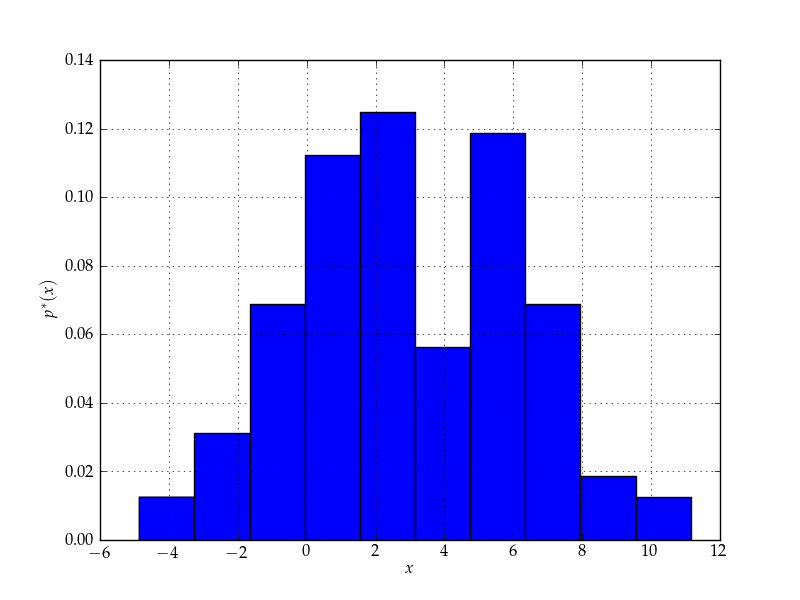
\includegraphics[width=1\linewidth]{pic/stat_series_eq_size.png}
  \caption{Равноинтервальная гистограмма распределения случайной величины $ X $\label{fig:eq-size_hist}}
\end{figure}

Вычислим значения интервального статистического ряда (таблица~\ref{tabl:eq-prob_int}) для построения
равновероятностной гистограммы (рисунок~\ref{fig:eq-prob_hist}).
\begin{table}[h!]
	\centering
	\caption{Равновероятностный статистический ряд\label{tabl:eq-prob_int}}
        \small
	\begin{tabular}{|c|c|c|c|c|c|c|}
		\hline
		$ j $	& $ A_j $	& $ B_j $	& $ h_j $	& $ v_j $	& $ p^{*}_j $	& $ f^{*}_j $ \\ \hline
1	& -4.860	& -0.905	& 3.955	& 10	& 0.1000	& 0.0253 \\ \hline
2	& -0.905	& 0.115	& 1.020	& 10	& 0.1000	& 0.0980 \\ \hline
3	& 0.115	& 1.210	& 1.095	& 10	& 0.1000	& 0.0913 \\ \hline
4	& 1.210	& 2.055	& 0.845	& 10	& 0.1000	& 0.1183 \\ \hline
5	& 2.055	& 2.600	& 0.545	& 10	& 0.1000	& 0.1835 \\ \hline
6	& 2.600	& 3.250	& 0.650	& 10	& 0.1000	& 0.1538 \\ \hline
7	& 3.250	& 5.190	& 1.940	& 10	& 0.1000	& 0.0515 \\ \hline
8	& 5.190	& 5.800	& 0.610	& 10	& 0.1000	& 0.1639 \\ \hline
9	& 5.800	& 7.150	& 1.350	& 10	& 0.1000	& 0.0741 \\ \hline
10	& 7.150	& 11.150	& 4.000	& 10	& 0.1000	& 0.0250 \\ \hline
Всего:	&	&	&16.010	&100	&1.0000	& \\ \hline

	\end{tabular}
\end{table}

\begin{figure}[h!]
  \centering
  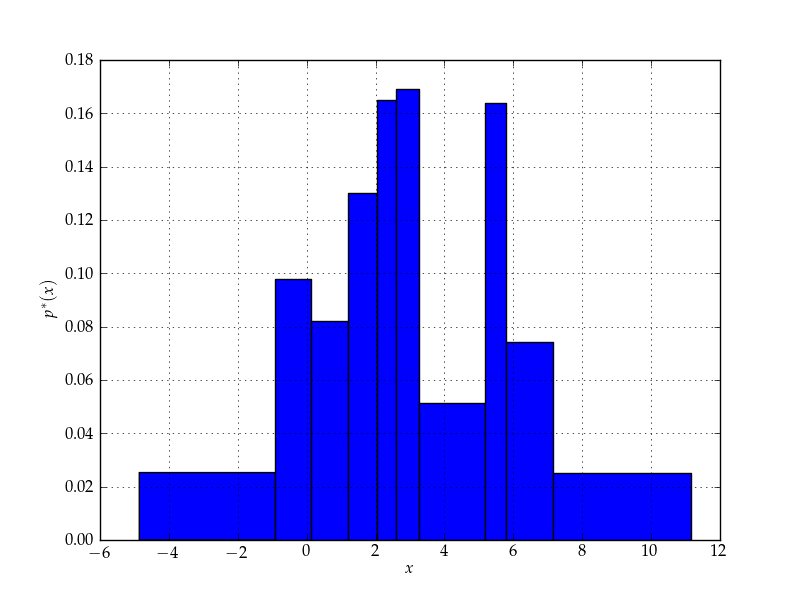
\includegraphics[width=1\linewidth]{pic/stat_series_eq_probability.png}
  \caption{Равновероятностная гистограмма распределения случайной величины $ X $\label{fig:eq-prob_hist}}
\end{figure}

\subsection{Вычисление оценок математического ожидания и дисперсии}

Запишем формулы для расчета cоответствующих оценок:
\begin{equation}
  m^*_X = \overline{x} = \frac{1}{n} \sum_{i=1}^{n} x_i,
\end{equation}

\begin{equation}
  I_\gamma(m_X) = \left[ \overline{x} - z_\gamma \dfrac{S_0}{\sqrt{n}};
    \overline{x} + z_\gamma \dfrac{S_0}{\sqrt{n}} \right],
\end{equation} 

\begin{equation}
  D^*_X = S^2_0 = \frac{1}{n-1} \sum_{i=1}^{n} x^2_i - \frac{n}{n-1} \overline{x}^2,
\end{equation}

\begin{equation}
  I_\gamma(D_X) = \left[ S_0^2 - z_\gamma \sqrt{ \dfrac{2}{n-1}} S_0^2;
    S_0^2 + z_\gamma \sqrt{ \dfrac{2}{n-1}} S_0^2 \right],
\end{equation} 

Результаты вычислений при $ \gamma = 0.95 $:
\begin{equation*}
	\begin{aligned}
		m^*_X &= 2.9967, &
		I_{0.95}(m_X) &= \left[ 2.3605; 3.6329 \right], \\
		D^*_X &= 10.5345, &
                I_{0.95}(D_X) &= \left[ 7.5998; 13.4692 \right].
	\end{aligned}
\end{equation*}

\newpage

\subsection{Выдвижение гипотезы о законе распределения случайной величины $ X $}
По виду графика эмпирической функции распределения $F^*(x)$ и гистограмм выдвинем один из следующих вариантов двухальтернативной
гипотезы о законе распределения случайной величины:
\begin{enumerate}

\item
	$H_0$ --- величина $X$ распределена по равномерному закону:
	\begin{equation}
		\begin{aligned}
			f(x)=
			\left\{
				\begin{aligned}
					&0, \hspace{11.5mm} x < a, \\
					&\frac{1}{b-a}, \hspace{2mm} a \le x \le b, \\
					&1, \hspace{11.5mm} x > b.
				\end{aligned}
			\right.
		\end{aligned}
	\end{equation}
	\begin{equation}
		\begin{aligned}
			F(x)=
			\left\{
				\begin{aligned}
					&0, \hspace{11.5mm} x < a, \\
					&\frac{x-a}{b-a}, \hspace{2mm} a \le x \le b, \\
					&1, \hspace{11.5mm} x > b.
				\end{aligned}
			\right.
		\end{aligned}
	\end{equation}
	$H_1$ --- величина $X$ не распределена по равномерному закону:
	\begin{align}
		f(x) & \neq f_0(x) ,&
		F(x) & \neq F_0(x).
	\end{align}

\item
	$H_0$ --- величина $X$ распределена по экспоненциальному закону:
	\begin{equation}
		\begin{aligned}
			&f(t)=
			\left\{
				\begin{aligned}
					&0, \hspace{11mm} t < 0, \\
					&\lambda e^{-\lambda t}, \hspace{2mm} a \le x \le b.
				\end{aligned}
			\right.
		\end{aligned}
	\end{equation}
	\begin{equation}
		\begin{aligned}
			&F(t)=
			\left\{
				\begin{aligned}
					&0, \hspace{17mm} t < 0, \\
					&1 - e^{-\lambda t}, \hspace{2mm} a \le x \le b.
				\end{aligned}
			\right.
		\end{aligned}
	\end{equation}
	$H_1$ --- величина $X$ не распределена по экспоненциальному закону:
	\begin{align}
		f(x) & \neq f_0(x) ,&
		F(x) & \neq F_0(x).
	\end{align}

\item
	$H_0$ --- величина $X$ распределена по нормальному закону:
	\begin{equation}
	  f(x) = f_0(x) = \frac{1}{\sigma\sqrt{2\pi}} \cdot \text{exp} \left[-\frac{(x-m)^2}{2\sigma^2} \right],
	\end{equation}
	\begin{equation}
	  F(x) = F_0(x) = 0.5 + \left( \frac{x-m}{\sigma} \right).
	\end{equation}
	$H_1$ --- величина $X$ не распределена по нормальному закону:
	\begin{align}
		f(x) & \neq f_0(x) ,&
		F(x) & \neq F_0(x).
	\end{align}
\end{enumerate}

В данном примере выдвинем двухальтернативную гипотезу о нормальном законе распределения случайной величины.

Учитывая, что $m^* = \overline{x} = 2.9967$ и $\sigma^* = \sqrt{D^*} = 3.2457$, получаем гипотетическую функцию распределения:

\begin{equation*}
  F_0(x) = 0,5 + \Phi \left( \frac{x-\overline{x}}{\sqrt{D^*}} \right) =
  0,5 + \Phi \left( \frac{x- 2.9967}{3.2457} \right)
\end{equation*}

Построим график $F_0(x)$ в одной системе координат с эмпирической функцией распределения $F^*(x)$ (рисунок~\ref{fig:sample_normal}). 

\newpage

\subsection{Проверка гипотезы о нормальном законе распределения 
  случайной величины $ X $ с помощью критерия Пирсона}

Вычислим значение критерия $\chi^2$ на основе равноинтервального статистического ряда
(таблица~\ref{tabl:eq-size_int}) по следующей формуле:
\begin{equation}
  \label{eq:chi^2}
	\chi^2 = n \sum_{j=1}^{10} \frac{(p_j-p^*_j)^2}{p_j}.
\end{equation}

Теоретические вероятности $p_j$ попадания в интервалы равноинтервального статистического ряда нормальной случайной величины с параметрами $m*$, $\sigma^*$ вычислим по следующей формуле:
\begin{equation*}
  p_j = F_0(B_j) - F_0(A_j) = \Phi \left( \frac{B_j + (2.9967)}{3.2457} \right) - \Phi \left( \frac{A_j + (2.9967)}{3.2457} \right).
\end{equation*}

Результаты расчетов приведены в таблице~\ref{tabl:pirson}.

\begin{table}[h!]
  \renewcommand{\arraystretch}{1.2}
  \renewcommand{\tabcolsep}{1.2em}
  \caption{Результаты расчетов значений слагаемых критерия $ \chi^2 $\label{tabl:pirson}}
  \centering
  \small
  \begin{tabular}{|c|c|c|c|c|c|c|c|}
    \hline
    $ j $	& $ A_j $	& $ B_j $	& $ F_0(A_j) $	& $ F_0(B_j) $	& $ p_j $	& $ p_j^{*} $	& $ \frac{(p^{*}_j - p_j)^2}{p_j} $ \\ \hline
1	& $ -\infty $	& -3.259	& 0.0000	& 0.0269	& 0.0269	& 0.0200	& 0.0018 \\ \hline
2	& -3.259	& -1.658	& 0.0269	& 0.0757	& 0.0487	& 0.0500	& 0.0000 \\ \hline
3	& -1.658	& -0.057	& 0.0757	& 0.1732	& 0.0975	& 0.1100	& 0.0016 \\ \hline
4	& -0.057	& 1.544	& 0.1732	& 0.3268	& 0.1536	& 0.1800	& 0.0045 \\ \hline
5	& 1.544	& 3.145	& 0.3268	& 0.5188	& 0.1921	& 0.2000	& 0.0003 \\ \hline
6	& 3.145	& 4.746	& 0.5188	& 0.7055	& 0.1866	& 0.0900	& 0.0500 \\ \hline
7	& 4.746	& 6.347	& 0.7055	& 0.8492	& 0.1438	& 0.1900	& 0.0149 \\ \hline
8	& 6.347	& 7.948	& 0.8492	& 0.9365	& 0.0873	& 0.1100	& 0.0059 \\ \hline
9	& 7.948	& 9.549	& 0.9365	& 0.9783	& 0.0418	& 0.0300	& 0.0033 \\ \hline
10	& 9.549	& $ +\infty $	& 0.9783	& 1.0000	& 0.0217	& 0.0200	& 0.0001 \\ \hline
	&	&	&	&Всего:	&1.0000	&1.0000	&0.0826 \\ \hline

  \end{tabular}
\end{table}

Проверим выполнение контрольного соотношения для $p_j$:
\begin{align}
	\left| 1 - \sum_{j=1}^{10} p_j \right| = value \le 0.01.
\end{align}

В cоответствии с формулой~\eqref{eq:chi^2} получаем $\chi^2= 100 \cdot 0.0826 = $ j $	& $ A_j $	& $ B_j $	& $ F_0(A_j) $	& $ F_0(B_j) $	& $ p_j $	& $ p_j^{*} $	& $ \frac{(p^{*}_j - p_j)^2}{p_j} $ \\ \hline
1	& $ -\infty $	& -3.259	& 0.0000	& 0.0269	& 0.0269	& 0.0200	& 0.0018 \\ \hline
2	& -3.259	& -1.658	& 0.0269	& 0.0757	& 0.0487	& 0.0500	& 0.0000 \\ \hline
3	& -1.658	& -0.057	& 0.0757	& 0.1732	& 0.0975	& 0.1100	& 0.0016 \\ \hline
4	& -0.057	& 1.544	& 0.1732	& 0.3268	& 0.1536	& 0.1800	& 0.0045 \\ \hline
5	& 1.544	& 3.145	& 0.3268	& 0.5188	& 0.1921	& 0.2000	& 0.0003 \\ \hline
6	& 3.145	& 4.746	& 0.5188	& 0.7055	& 0.1866	& 0.0900	& 0.0500 \\ \hline
7	& 4.746	& 6.347	& 0.7055	& 0.8492	& 0.1438	& 0.1900	& 0.0149 \\ \hline
8	& 6.347	& 7.948	& 0.8492	& 0.9365	& 0.0873	& 0.1100	& 0.0059 \\ \hline
9	& 7.948	& 9.549	& 0.9365	& 0.9783	& 0.0418	& 0.0300	& 0.0033 \\ \hline
10	& 9.549	& $ +\infty $	& 0.9783	& 1.0000	& 0.0217	& 0.0200	& 0.0001 \\ \hline
	&	&	&	&Всего:	&1.0000	&1.0000	&0.0826 \\ \hline
 $.

Вычислим число степеней свободы: $ k = M - 1 - s = 10 - 1 - 2 = 7 $. 

По заданному уровню значимости ($\alpha = 0.05$) из таблицы распределения $\chi^2$ выбирем критическое значение:
\begin{equation*}
  \chi^2_{\alpha; k} = \chi^2_{0.05; 7} = 14.07.
\end{equation*}

\textbf{Вывод:} так как $\chi^2 = $ j $	& $ A_j $	& $ B_j $	& $ F_0(A_j) $	& $ F_0(B_j) $	& $ p_j $	& $ p_j^{*} $	& $ \frac{(p^{*}_j - p_j)^2}{p_j} $ \\ \hline
1	& $ -\infty $	& -3.259	& 0.0000	& 0.0269	& 0.0269	& 0.0200	& 0.0018 \\ \hline
2	& -3.259	& -1.658	& 0.0269	& 0.0757	& 0.0487	& 0.0500	& 0.0000 \\ \hline
3	& -1.658	& -0.057	& 0.0757	& 0.1732	& 0.0975	& 0.1100	& 0.0016 \\ \hline
4	& -0.057	& 1.544	& 0.1732	& 0.3268	& 0.1536	& 0.1800	& 0.0045 \\ \hline
5	& 1.544	& 3.145	& 0.3268	& 0.5188	& 0.1921	& 0.2000	& 0.0003 \\ \hline
6	& 3.145	& 4.746	& 0.5188	& 0.7055	& 0.1866	& 0.0900	& 0.0500 \\ \hline
7	& 4.746	& 6.347	& 0.7055	& 0.8492	& 0.1438	& 0.1900	& 0.0149 \\ \hline
8	& 6.347	& 7.948	& 0.8492	& 0.9365	& 0.0873	& 0.1100	& 0.0059 \\ \hline
9	& 7.948	& 9.549	& 0.9365	& 0.9783	& 0.0418	& 0.0300	& 0.0033 \\ \hline
10	& 9.549	& $ +\infty $	& 0.9783	& 1.0000	& 0.0217	& 0.0200	& 0.0001 \\ \hline
	&	&	&	&Всего:	&1.0000	&1.0000	&0.0826 \\ \hline
 {<}sign{>} \chi^2_{0.05;7} $, то гипотеза $H_0$ о нормальном законе распределения принимается (отклоняется). 


\subsection{Проверка гипотезы о нормальном законе распределения 
  случайной величины $ X $ с помощью критерия Колмогорова}

По рисунку~\ref{fig:sample_normal} определим максимальное по модулю отклонение между функциями $F^*(x)$ и $F_0(x)$:
\begin{align}
	Z = \max_{i=1}^n \Big| F^*(x_i) - F_0(x_i) \Big| = 0.0777.
\end{align}

Вычислим значение критерия Колмогорова по формуле:
\begin{align}
  \lambda &= \sqrt{n} \cdot Z, \\ \nonumber
  \lambda &= \sqrt{100} \cdot 0.0777 = 0.7767.
\end{align}

Из таблицы <<критических значений>> для критерия Колмогорова по заданному уровню значимости ($\alpha = 0.05$)
выбираем критическое значение $\lambda_{\gamma} = \lambda_{1-\alpha} = \lambda_{0.95} = 1.36 $.

\textbf{Вывод:} так как $\lambda = 0.7767 {<}notation{>} \lambda_{0.95} $, то гипотеза $H_0$ о нормальном законе распределения принимается (отклоняется).

\newpage
\fancyhf{}
\newgeometry{left=1cm,right=1cm,top=1cm}
\begin{landscape}
  \begin{figure}[H]
    \centering
    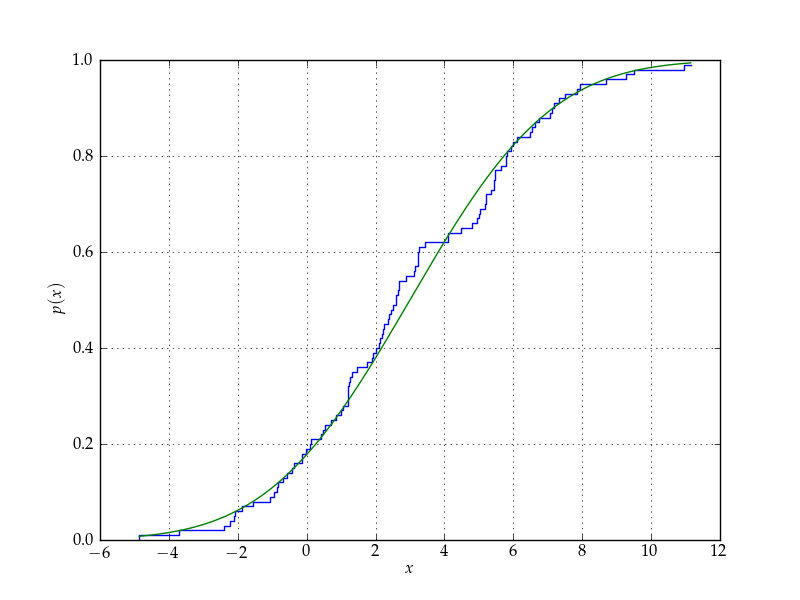
\includegraphics[width=0.9\linewidth]{pic/sample_normal.png}
    \caption{График гипотетической и эмпирической функций распределения случайной величины $ X $\label{fig:sample_normal}}
  \end{figure}
\end{landscape}
\restoregeometry

\end{document}